\RequirePackage{plautopatch}
% 一応pLaTeX用パッチを当てておく
% クラスオプションでdvipdfmxを読み込めばusepackageで個別に指定する必要がなくなる
% jarticleは非推奨なので使いたくないが、レギュレーションなので大変遺憾に思いつつ従う
\documentclass[dvipdfmx,12pt,a4j]{jarticle}
% dvipdfmxはグローバルオプションとして読み込んでいるので不要
\usepackage{graphicx}
% ロゴ関係
\usepackage{bxtexlogo}
\bxtexlogoimport{*,**}
% Hオプションを使いたいので読み込む
\usepackage{here}
% ソースコードを表示するのに読み込む
\usepackage{listings}
% シンタックスハイライトのため
\usepackage{xcolor}
% 枠かこみのため
\usepackage{tcolorbox}
% url挿入のため
\usepackage{url}
% xcolorの色定義
\definecolor{solarized@base03}{HTML}{002B36}
\definecolor{solarized@base02}{HTML}{073642}
\definecolor{solarized@base01}{HTML}{586e75}
\definecolor{solarized@base00}{HTML}{657b83}
\definecolor{solarized@base0}{HTML}{839496}
\definecolor{solarized@base1}{HTML}{93a1a1}
\definecolor{solarized@base2}{HTML}{EEE8D5}
\definecolor{solarized@base3}{HTML}{FDF6E3}
\definecolor{solarized@yellow}{HTML}{B58900}
\definecolor{solarized@orange}{HTML}{CB4B16}
\definecolor{solarized@red}{HTML}{DC322F}
\definecolor{solarized@magenta}{HTML}{D33682}
\definecolor{solarized@violet}{HTML}{6C71C4}
\definecolor{solarized@blue}{HTML}{268BD2}
\definecolor{solarized@cyan}{HTML}{2AA198}
\definecolor{solarized@green}{HTML}{859900}
% listingsのスタイル定義
\lstdefinestyle{c}{
  language=c,
  numbers=left
}
\lstset{
basicstyle=\small\ttfamily\color{solarized@base00},
rulesepcolor=\color{solarized@base03},
numberstyle=\scriptsize\color{solarized@base01},
keywordstyle=\color{solarized@blue},
stringstyle=\color{solarized@cyan}\ttfamily,
commentstyle=\color{solarized@base01},
emphstyle=\color{solarized@red},
backgroundcolor=\color{solarized@base3},
sensitive=true,
breaklines=true,
breakatwhitespace=true,
framerule=0pt,
frame=l
showstringspaces=false,
tabsize=2,
basewidth={0.57em,0.52em},
}
\title{プログラミング 第1回レポート}
\author{202111609 仲村和士}
\date{\today}

\begin{document}
\maketitle
\section{はじめに}
課題内容を始める前に重要なことを何点かこの節で述べる。

\subsection{\BibTeX のコンパイルについて(重要)}
はじめに本レポートをコンパイルする際の注意点について述べたい。本レポートの文献情報には日本語書籍が含まれている。したがって通常の\BibTeX ではなく\pBibTeX を利用することを推奨する。
\begin{verbatim}
  $ pbibtex -kanji=utf-8 file_name
\end{verbatim}

\subsection{\LaTeX 利用の方針}
随時インターネットで調べた結果を活用するが、日本語\LaTeX の代表的書籍である、奥村、黒木~\cite{bibunsho}に記述があるものはこれに従う。講義資料と齟齬がある点についてはその都度記述する。

ただし、例外的にjarticleを利用する点のみ前述の書籍の記述から外れるものとする。\LaTeX の作法としては非推奨であるが、今回のレポートのレギュレーションである以上それに従うものとする。

\section{Linuxのコマンド利用}

\section{ソースコードの挿入}
\subsection{課題内容と方針}\label{sec:code}
本課題は与えられたC言語のソースコードを図として掲載するという内容である。もっとも簡単な方法はverbatim環境を利用することであるが、ここではlistingパッケージを利用してよりきれいなリストの作成を試みる。listingsパッケージの用法については情報科学類~\cite[p.183]{tebiki}による。また、オプションのつけ方に関しては~\cite{listing}も参照した。
listingパッケージの利用方法を簡単に述べておくと、まず、プリアンブルで\verb|\lstdefinestyle|を用いてスタイルを定義する。その際、複数のスタイルを定義できるが、共通の設定に関しては\verb|\lstset|に記述するとコンパクトである。ここまででlistingsパッケージを利用する準備が整った。listingsの利用方法は次の3種類である。
\begin{enumerate}
  \item \LaTeX ソースに直接埋め込む
  \item ファイルから読み込む \label{enum:listing}
  \item インラインで挿入する
\end{enumerate}
今回はファイルが与えられているので\ref{enum:listing}の方法を採用する。
この方法では\verb|\lstinputlisting|コマンドを利用する。

\subsection{実際に挿入する}
\ref{sec:code}節で方針を説明したので、それの通りにソースコードを挿入する。
Listing \ref{lst:sort}はC言語によるソートの実装例である。
\lstinputlisting[caption=バブルソートの実装例,label=lst:sort,style=c]{./sort.c}
\subsection{確認}
Listing \ref{lst:sort}は行番号がつけられており、画像ではない図として挿入されている。よって題意を満たしている。

\section{画像の挿入}
\subsection{課題内容と方針}\label{subsection:方針}

本課題は全学計算機を操作しているコマンドラインをキャプチャして、画像を図として挿入するという内容である。
私の環境はWindowsであるから、画像のキャプチャには[Win]+[Shift]+sで開始される「切り取り\&スケッチ」の機能を利用する。
画像を挿入するにはgraphicxパッケージの\verb|\includegraphics|コマンドを利用する。図として挿入するためにはfigure環境を用いる。本レポートではHオプションを利用するためにhereパッケージも読み込んでいる。

ここで、graphicxの注意点について述べておく。講義資料ではPNGを埋め込むためには.xbbファイルが必要と記されているが、それは旧情報である。現在ではこのようなファイルは不要であり、むしろ誤動作の原因となるので消しておくのが安全である。\cite[p.126]{bibunsho}

\subsection{実際に挿入する}\label{subsection:実際に挿入する}
図\ref{fig:keisanki}は全学計算機を使っている様子である。この図の中で行っていることを順番に説明する。

最初のlと書かれた部分ではエイリアスが利用できることを確認している。.bashrcにエイリアスが書いてあり、lsの代わりにlで動作するようになっている。次のechoではaliasが便利であるということを標準入出力を利用して主張している。次のls \verb+|+ wcではホームディレクトリをlsで調べた結果をパイプでwcに渡して行数、単語数、文字数を調べている。深い意味はない。次の man man \verb+|+ cat \verb+|+ wcはパイプを連鎖的に用いたワンライナーであり、manコマンドのマニュアルをcatでまとめて標準出力に流し、wcで大体のボリュームを確認している。次のコマンドlualatexでは、lualatexが利用できるということを確認している。この実行結果により、副次的にTeX Liveのバージョンが2021であり、ほぼ最新の環境が利用できるということが分かった。次のechoではその旨を主張しているが、リダイレクトでファイルに保存している。ファイル名はArch is the bestプロジェクト\footnote{Arch Linuxの優位性を示すための、少々思想が強いプロジェクト。ArchWikiに多くのプログラミング言語による実行方法が記載されている。}のパロディである。最後のechoでは、この画像が何をしているところなのかを示している。
\begin{figure}[H]
  \centering
  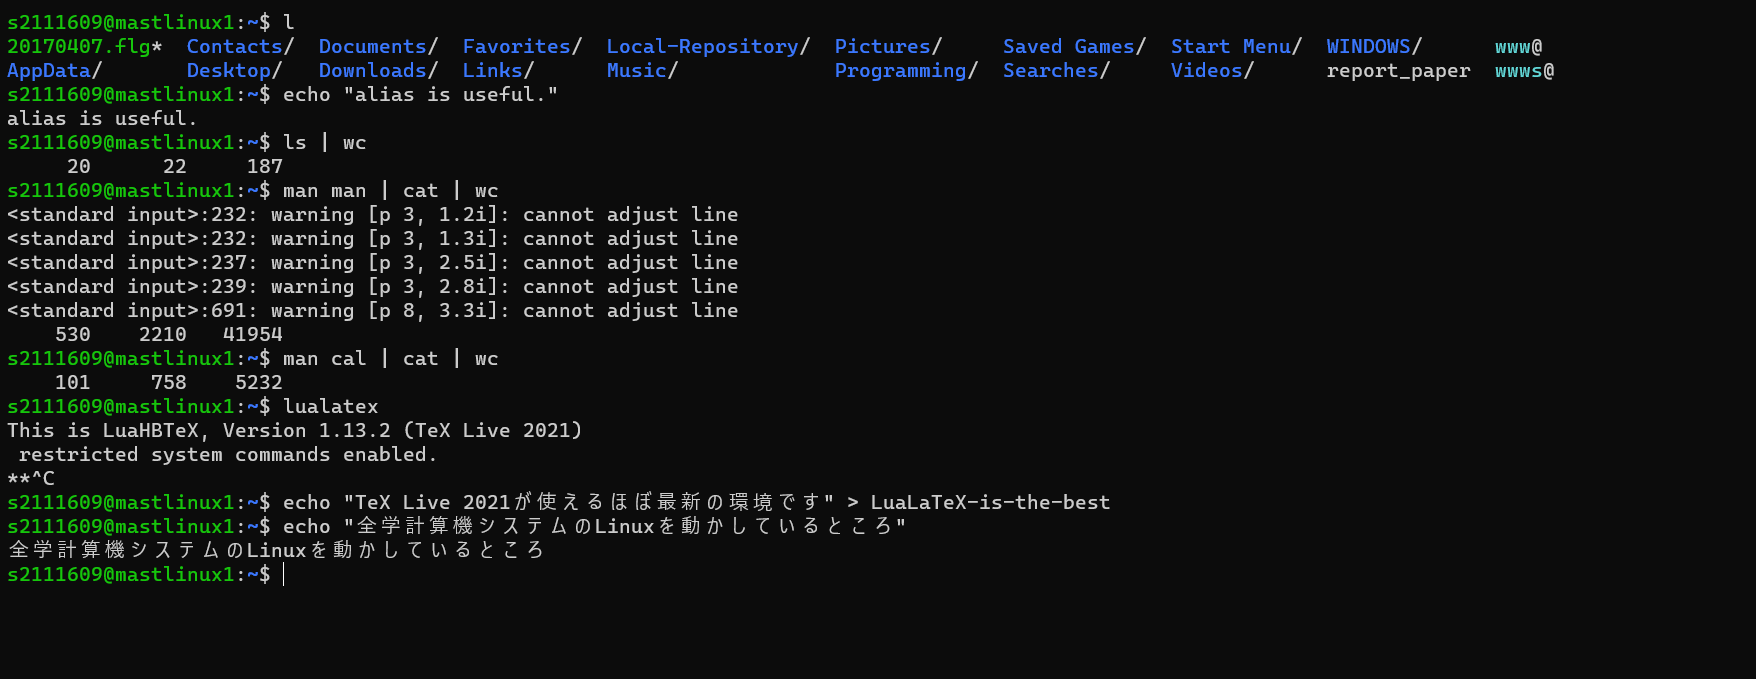
\includegraphics[width=15cm]{imgs/commandline.png}
  \caption{全学計算機を使っているところ}
  \label{fig:keisanki}
\end{figure}

\subsection{確認}
本節の指示内容は次の通りであった。
\begin{enumerate}
  \item キャプチャ方法を含めて、上述の内容を達成した方法を記述する \label{enum:how}
  \item 全学計算機システムを利用しているところをキャプチャして図として挿入する\label{enum:figure}
  \item 図の内部で何をしているのかを説明する\label{enum:explain}
\end{enumerate}
\ref{enum:how}は\ref{subsection:方針}節で記述した。\ref{enum:figure}と\ref{enum:explain}は\ref{subsection:実際に挿入する}節で記述した。よって題意を満たしている。
\section{本の紹介}
\subsection{概略}
本節では私の好きな本および、私が世話になった本を紹介したい。私の本棚の本は専門書/技術書が大半を占めているが、それでは面白くないため後半では意図的に技術書ではない本をを2冊紹介することにした。
前半の2冊が世話になった本で後半2冊が好きな本(非技術書)である。
\begin{itemize}
  \item \LaTeXe 美文書作成入門 改訂第8版 ~\cite{bibunsho}
  \item ホログラフィ入門: コンピュータを利用した3次元映像・3次元計測~\cite{holo-nyumon} 
  \item 三日間の幸福~\cite{koufuku}
  \item 恋する小惑星~\cite{koiasu}
\end{itemize}

\subsection{本の内容紹介}
\LaTeXe 美文書作成入門 改訂第8版 ~\cite{bibunsho}は言わずと知れた日本語\LaTeX の大ベストセラー書籍の最新版である。\LaTeX を活用する上で必要なほぼすべてのトピックが網羅されており、日常的に\LaTeX を利用する人は通読したうえで信頼性の高いリファレンスとして手元に置くべき一冊である。

ホログラフィ入門: コンピュータを利用した3次元映像・3次元計測~\cite{holo-nyumon} は私が1年次のAREのときに大変世話になった本であり、ホログラフィの概念、および波動光学を利用した回折計算法などが実装とともに解説されている実用的な一冊である。

三日間の幸福~\cite{koufuku}はWeb発の小説であり、金欠学生の主人公が寿命を売れるという噂を聞き、査定を依頼するが、最低買取価格である1万円/年を言い渡され、生きる気力を失った主人公が残り3カ月を残してすべて売るというシーンから始まる。彼がどのような3カ月を過ごすのか—ぜひ手にとってみてほしい。

恋する小惑星~\cite{koiasu}はまんがタイムきららキャラットに連載された漫画である。「小惑星を見つけたい」という夢を持った高校生の主人公を中心に地質、地図、気象などさまざまな地学の分野に興味をもつ地学系女子たちによる物語である。つくばは本作品の聖地であるから、筑波大学の学生は必見である。
\subsection{確認}
本節での指示内容は以下の通りである。
\begin{itemize}
  \item 課題フォームに記載された構成を満たす
  \item 本をitemize環境で列挙し、文献を参照する
  \item 文献を参照しつつ、100字程度でそれぞれの本の説明を書く
\end{itemize}
本節ではこれらをすべて満たしている。よって設問の題意を満たしていることが確認できた。

\bibliographystyle{junsrt}
\bibliography{citation}
\end{document}
